%VD: a subheading immediately after a headng should be avoided
%\subsection{Setup}
Since deep reinforcement learning algorithms need millions of iterations to train, in the absence of thousands of robotic replicas like \cite{LePaKrISER2017}, we evaluate the algorithms on a simulated environment.
We use the same game engine as \cite{MiPaViICLR2017}, called Deepmind Lab (\cite{BeLeTeARXIV2016}).
The game is setup such that an agent is placed within a randomly generated maze containing a \emph{goal} at a particular location.
On reaching the goal, the agent \emph{re-spawns} within the same maze while the goal location remains unchanged. 
Following \cite{MiPaViICLR2017}, we scatter the maze with randomly placed smaller apple rewards (+1) to encourage initial explorations and assign the goal a reward of +10.
% VD: Defining the objective in terms of reward is wrong because designing rewards is a part of reinforcement learning not the problem statement.
The agent is tasked to find the goal as many times as possible within a fixed amount of time, re-spawning within the maze, either statically or randomly, each time it reaches the goal.
% JJC: TODO: remind that the spawn location can be random or static

Unlike \cite{MiPaViICLR2017}, we include a small wall penalty (-0.2) that pushes the agent away from the wall.
% VD: Do we need experiments to support that?
% VD: It is not clear how wall penality will avoid backward motion. Let's avoid that argument.
The wall penalty is useful to prevent agents from moving along the walls, thereby discarding vision input for exploration.
% Reward formulation
%The setup of game is such that it enables evaluating the algorithm for optimal path planning as well as enable dividing experiments into exploration and exploitation stages.
%We introduce a metric that evaluates how well the agent exploits the information gained during exploration before finding the goal for the first time.
% The optimal way of finding the goal in fastest way is to collect
% enough information for creating a map and use the map to find the shortest path from start to end location.
% However, an end-to-end navigation algorithm might find other ways of finding optimal strategies to find the goal.
We also use a discrete 4-action space (move forward/backward, rotate left/right)which is different from the 8-action space one used by \cite{MiPaViICLR2017}.
% VD: Do we need to show experiments for these claims?
% JJC: TODO: explain why this won't effect the comparability of results.
A smaller action space helps the algorithm train faster while achieving similar reward values.
% VD: this will raise more questions like why grounding in vision is necesary
% The agent's picking up of rewards is thus explicitly grounded in its vision as the agent must rotate in the direction of motion during exploration.

We generate 1100 random maps using depth-first search based maze generation methods.
More information on maze generation can be found in the appendix. 
Of the first 1000 maps, 10 are randomly selected for our static-map experiments (Fig. \ref{fig:environments}). For our unseen map experiments, agents are trained on increasing subsets of the first 1000 maps and tested on the remaining 100.
Unlike \cite{MiPaViICLR2017} and similar to \cite{ChLaSaNIPS2016}, we use randomly textured walls in our mazes so that the policies learned are texture-independent.

\paragraph{Evaluation Metrics}
We evaluate the performance in terms of three meteric: rewards, ratio of distance traveled to shortest distance and \LatencyOneGtOne{}.
For all the experiments we compute mean and standard deviation over 100 episodes.
\begin{itemize}
\item The total reward per episode 
\item We also compute the ratio of total distance traveled by the agent to the sum of approximate shortest distances to the goal. The shortest distance between the spawn point and goal location is computed in the block world and hence is only an approximation of the shortest distance. 
\item 
\end{itemize}

% VD: Let's describe this terminology in the descriptions of tasks
% Througout our experiments we refer to goal locations, spawn locations and maps as static or random.
% When static is used for spawn and goal location, they described positions that remain fixed through all episodes during both the training and the testing.
% When random is used, the spawn location changes randomly throughout the duration of the episode for both training and testing. When used for the goal, random means that its locations changes between episodes for training and testing. During the course of an episode, however, a random goal remains in the same position allowing for agents that exploit map information to find it repeatedly and thus maximize reward.
% In the context of maps, statics maps imply that the same map is used for training and testing. Random means that agents are simulataneously trained on multiple maps and tested on previously unseen ones.

\subsection{Experiments}
\label{sec:navtasks}
We evaluate the Nav-A3C algorithm on maps with 5 stages of difficulty. While the Nav-A3C algorithm works smoothly on the easier stages, it does not perform better than bug-exploration methods on the hardest stage.
We propose these experiments as a 5-stage benchmark for all end-to-end navigation algorithms.

%While there already exists optimal algorithms to find shortest path between two points and perform optimal navigation between given set of points in a given map, the advantage of Deep reinforcement learning comes from its ability to extract required features from the input images and its promise
%optimize mapping and path planning in end-to-end fashion. 
%Thus we need to either integrate existing path planning and mapping methods with deep learning methods to perform end-to-end training or extend deep learning methods to learn path planning and mapping.

\begin{description}
  \ditem{Static goal, static spawn, and static map}
  \label{prob:sss}
  % VD: Ask people if the name of the experiment makes it clear
  %In this setup, we keep the goal location, spawn location and the map fixed during both training and testing.
  %This is the easiest variation of our experiments with the environment being deterministic. 
  To perform optimally on this experiment, the agent needs to find and learn the shortest path at training time and repeat it during testing. 

  \ditem{Static goal, random spawn and static map}
  % VD: Probably clear from the name
  % In this setup, we keep the goal location and the map fixed during both training and testing but chose a random spawn point every time the agents re-spawns.
  This is a textbook version of the reinforcement learning problem, especially in gridworld \cite{SuBaBOOK1998}, with the only difference being that the environment is partially observable instead of fully observable.
  This problem is more difficult than Problem~\ref{prob:sss} because the agent
  must find an optimal policy to the goal from each possible starting point in the maze.
  \ditem{Random goal, static spawn, and static map}
  % VD: The randomness of the goal is what we need to qualify
  In this setup, we keep the spawn location and the map fixed during both training and testing but chose a random goal location for each episode.
  Note that the goal location stays constant throughout an episode.
  % VD: This line does not add any information
  %This experiments highlights the map-exploitation ability of the agent.
  The agent can perform well on this experiment, by remembering the goal location after it has been discovered and exploiting the information to revisit goal faster.  
  
  Following \cite{MiPaViICLR2017}, we report the ratio
  of time taken to hit the goal for the first time (exploration time) vs the average amount of time taken to hit goal subsequently (exploitation time). The metric, called \emph{\LatencyOneGtOne{}}, is a measure of how efficiently the agent exploits map information to find shorter path once the goal location is known. 
  If this ratio is greater than 1, then we say that the agent is doing better than random exploration and higher values is better.
  \ditem{Random goal, random spawn, and static map}
  In this version of the experiment both the spawn point and the goal location is randomized. To perform optimally, the agent must localize itself within the map in addition to being able to exploit map-information.
  
  This is the problem that is addressed by \cite{MiPaViICLR2017} with limited success. 
  They evaluate this case on two maps and report \LatencyOneGtOne{} to be greater than 1 in one of the two maps. We evaluate the same metric on ten other maps and provide the tools for application to several more.
  \ditem{Random goal, random spawn, and random map}
    We believe that any proposed algorithms on end-to-end navigation problems, should be evaluated on unseen maps.
    To our knowledge, this is the first paper to do so in the case of deep reinforcement learning based navigation methods.
    We train agents to simultaneously learn to explore 1, 10, 100, 500 and 1000 maps and test them on the same 100 unseen maps. The relevant results can be found in Fig~\ref{fig:num-training-maps} and discussed in Section~\ref{sec:analysis}.
\end{description}

The comparative evaluation of the different the stages of this benchmark are shown in Fig~\ref{fig:latency-goal-reward} and expanded upon in the next section.

%\subsection{Evaluation Maps}
%We evaluate our trained models on a few qualitative maps previously unseen during training time. Each of these maps have two paths to the goal. 
%We evaluate the percentage of times the agent travels to the goal along the shortest path after discovering it in the exploitation phase. 
%The purpose of these maps is to quantitavely evaluate whether these trained models can translate map-exploitative abilities to new, unseen maps. 
%
%\setcounter{Benchmark}{0}
%\begin{description}
%    \ditem{Square Map}
%        
%    \ditem{Wrench map}
%    This map is shown on the top row, extreme right column in Fig~\ref{fig:environments}. It has one loop and a corridor.
%    The goal is placed asymmetrically in the loop and the agent is spawned in the corridor.
%    Because of asymmetrical placement of the goal, one of the path to the goal is shorter than the other and there are only two possible paths.
%    We record the path taken each time. If the agent has learned a greedy strategy, then it would repeat the path taken for the first time.
%    We evaluate the fraction of times, the agent repeats the first path. A higher number indicates a greedy strategy.
%    In second evaluation, we let the agent explore randomly untill it hits the goal via the shorterst path.
%    At this point we evaluate the  fraction of times shortest path is taken. For this score 
%    \ditem{Goal map}
%    This map is shown on the bottom row, extreme right column in Fig~\ref{fig:environments}.
%    We chose this map because this is the simplest map with a fork. Making the map any simpler will make the map homeomorphic to a straight line. 
%    We evaluate the number of times the agent takes the right descision at the fork after exploring the goal once.
%\end{description}

% \begin{figure}%
% 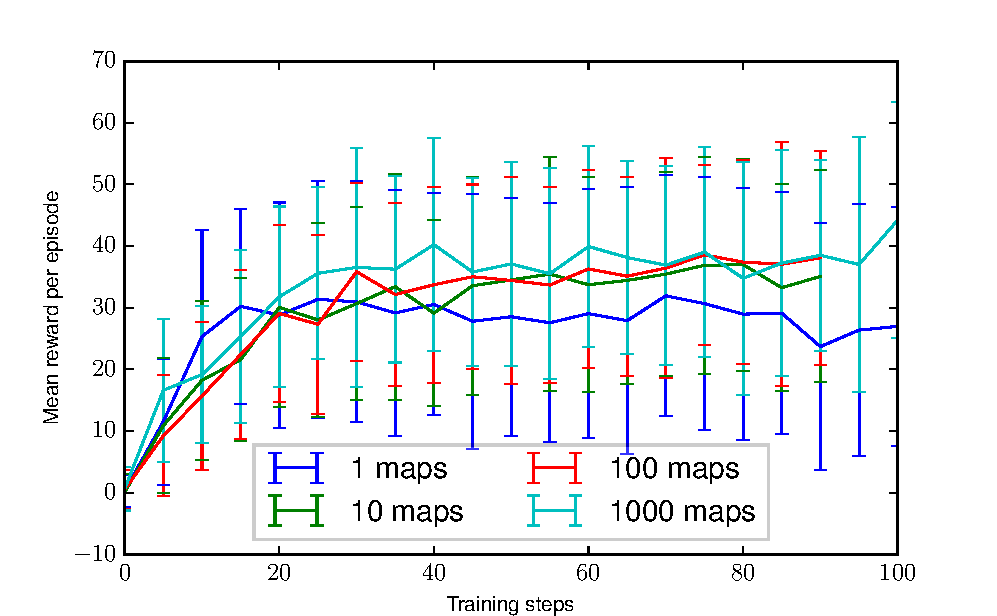
\includegraphics[width=0.5\columnwidth]{images/plot_reward_3D-1000.pdf}%
% 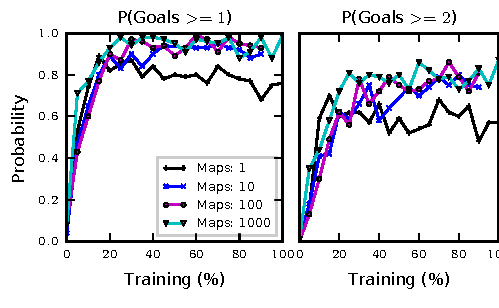
\includegraphics[width=0.5\columnwidth]{images/plot_probability_3D-1000.pdf}%
% \vspace{-1em}%
% \caption{Mean reward while tested on 100 unseen maps, while being trained on different number of training maps. Note that while training on 1000 maps eventually achieves high reward, it is only higher mean reward (44.2), training on 1 map hits the maximum (31) much faster.}%
% \label{fig:plot_reward_on_testing}%
% \end{figure}


%We evaluate the Nav-A3C\cite{MiPaViICLR2017} algorithm on randomly chosen ten maps with increasing difficulty.
%The results of our experiments are shown in Fig~\ref{fig:latency-goal-reward}.
%We change the randomness of either the spawn point or the goal location.
%We note that the increasing randomness gradually reduce the maximum reward achived and the number of times the goal is reached. As expected, the variance in reward and number of times goals is reached also increases with randomless.
%

%\subsection{Evaluation Metrics}
%We report three evaluation metrics in all our experiments: reward, average number of goal hits and \LatencyOneGtOne{}. We run evaluations on a map for 100 episodes and take the mean and standard deviation of the rewards per episode and number of goal hits per episode. Even though reward includes rewards due to apples and negative rewards due to wall penalities, the reward due to goal dominates dominates the reward metric making reward approximately ten times the average goal hits.
%
%The \LatencyOneGtOne{} is defined as the ratio of time take to find the goal first time to the average time take to find goal thereafter.
%Note that whenever the goal location is ``Random'' (different in each episode but same for the episode), untill the goal is found for the first time, the agent is just exploring the map.
%After the first goal hit, the agent should be able to exploit the location of the goal to find the goal in shorter times.
%Hence a \LatencyOneGtOne{} value greater than one indicates that the algorithm is able to successfully exploit information gathered during goal finding exploration.
%
